\documentclass[tikz,border=8pt]{standalone}
\usepackage{tikz}
\usetikzlibrary{arrows.meta,positioning,fit,calc}

\begin{document}
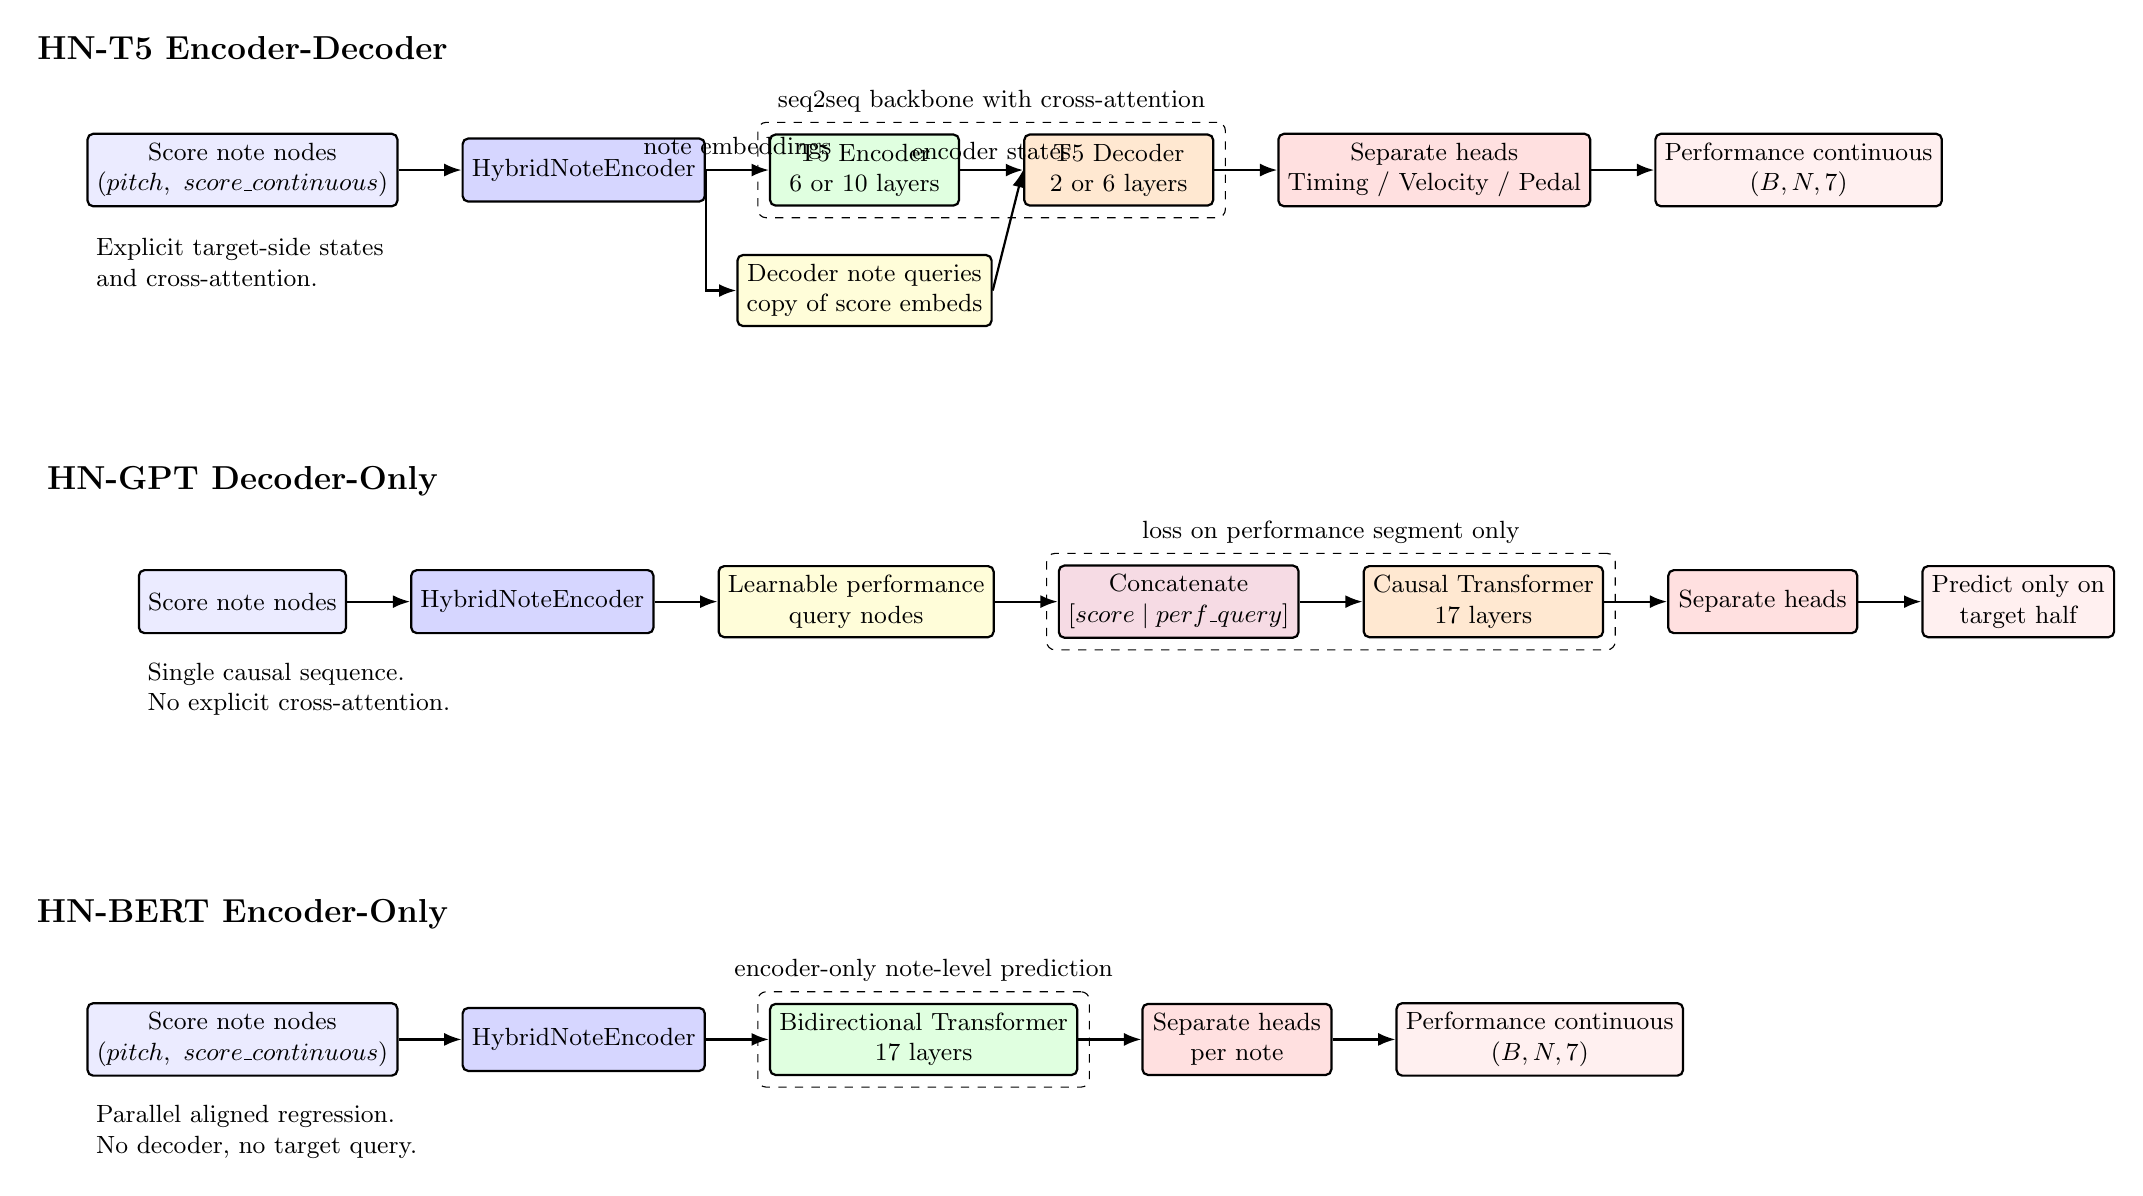
\begin{tikzpicture}[
  font=\small,
  node distance=6mm and 8mm,
  box/.style={
    draw,
    rounded corners=2pt,
    thick,
    align=center,
    minimum height=8mm,
    minimum width=24mm
  },
  title/.style={font=\bfseries\large},
  flow/.style={-{Latex[length=2.2mm]}, thick},
  group/.style={draw, dashed, rounded corners=3pt, inner sep=4pt},
  note/.style={align=left, font=\small}
]

% Panel A: T5
\node[title] (t5title) at (0, 0) {HN-T5 Encoder-Decoder};
\node[box, fill=blue!8, below=8mm of t5title] (t5score) {Score note nodes\\$(pitch,\ score\_continuous)$};
\node[box, fill=blue!16, right=of t5score] (t5encemb) {HybridNoteEncoder};
\node[box, fill=green!12, right=of t5encemb] (t5enc) {T5 Encoder\\6 or 10 layers};
\node[box, fill=yellow!15, below=of t5enc] (t5query) {Decoder note queries\\copy of score embeds};
\node[box, fill=orange!18, right=of t5enc] (t5dec) {T5 Decoder\\2 or 6 layers};
\node[box, fill=red!12, right=of t5dec] (t5head) {Separate heads\\Timing / Velocity / Pedal};
\node[box, fill=red!6, right=of t5head] (t5out) {Performance continuous\\$(B,N,7)$};
\node[note, below=7mm of t5score.south west, anchor=west] (t5note) {Explicit target-side states\\and cross-attention.};

\draw[flow] (t5score) -- (t5encemb);
\draw[flow] (t5encemb) -- node[above] {note embeddings} (t5enc);
\draw[flow] (t5encemb.east) |- (t5query.west);
\draw[flow] (t5query.east) -- (t5dec.west);
\draw[flow] (t5enc.east) -- node[above] {encoder states} (t5dec.west);
\draw[flow] (t5dec) -- (t5head);
\draw[flow] (t5head) -- (t5out);
\node[group, fit=(t5enc)(t5dec), label=above:{seq2seq backbone with cross-attention}] {};

% Panel B: GPT
\node[title] (gpttitle) at (0, -55mm) {HN-GPT Decoder-Only};
\node[box, fill=blue!8, below=8mm of gpttitle] (gptscore) {Score note nodes};
\node[box, fill=blue!16, right=of gptscore] (gptencemb) {HybridNoteEncoder};
\node[box, fill=yellow!15, right=of gptencemb] (gptquery) {Learnable performance\\query nodes};
\node[box, fill=purple!14, right=of gptquery] (gptconcat) {Concatenate\\$[score \mid perf\_query]$};
\node[box, fill=orange!18, right=of gptconcat] (gptbackbone) {Causal Transformer\\17 layers};
\node[box, fill=red!12, right=of gptbackbone] (gpthead) {Separate heads};
\node[box, fill=red!6, right=of gpthead] (gptout) {Predict only on\\target half};
\node[note, below=7mm of gptscore.south west, anchor=west] (gptnote) {Single causal sequence.\\No explicit cross-attention.};

\draw[flow] (gptscore) -- (gptencemb);
\draw[flow] (gptencemb) -- (gptquery);
\draw[flow] (gptquery) -- (gptconcat);
\draw[flow] (gptconcat) -- (gptbackbone);
\draw[flow] (gptbackbone) -- (gpthead);
\draw[flow] (gpthead) -- (gptout);
\node[group, fit=(gptconcat)(gptbackbone), label=above:{loss on performance segment only}] {};

% Panel C: BERT
\node[title] (berttitle) at (0, -110mm) {HN-BERT Encoder-Only};
\node[box, fill=blue!8, below=8mm of berttitle] (bertscore) {Score note nodes\\$(pitch,\ score\_continuous)$};
\node[box, fill=blue!16, right=of bertscore] (bertencemb) {HybridNoteEncoder};
\node[box, fill=green!12, right=of bertencemb] (bertbackbone) {Bidirectional Transformer\\17 layers};
\node[box, fill=red!12, right=of bertbackbone] (berthead) {Separate heads\\per note};
\node[box, fill=red!6, right=of berthead] (bertout) {Performance continuous\\$(B,N,7)$};
\node[note, below=7mm of bertscore.south west, anchor=west] (bertnote) {Parallel aligned regression.\\No decoder, no target query.};

\draw[flow] (bertscore) -- (bertencemb);
\draw[flow] (bertencemb) -- (bertbackbone);
\draw[flow] (bertbackbone) -- (berthead);
\draw[flow] (berthead) -- (bertout);
\node[group, fit=(bertbackbone), label=above:{encoder-only note-level prediction}] {};

\end{tikzpicture}
\end{document}
